\documentclass[a4paper]{article}
%\documentclass[a4paper,twocolumn]{article}
%\documentclass[a4paper,landscape,twocolumn]{article}
%\documentclass[a4paper]{memoir}
\usepackage[utf8]{inputenc}
\usepackage[spanish, es-tabla, es-nodecimaldot]{babel}
%\usepackage[english]{babel}
\usepackage{amsmath}  %permite usar \text{} en el entorno Matemática
\usepackage{amssymb} % para el de números reales
%\usepackage{fancyhdr} %para encabezados y pies de página lindos
%\usepackage{lastpage} %para poder referenciar el número de la última página
\usepackage{graphicx} %para insertar gráficos
\usepackage{float} %para que funcione el H de la posición de las figuras
%\usepackage{chngpage} %para cambiar márgenes temporalmente. Por ejemplo tabla o figura un poco más grande que el text width
%\usepackage[format=plain, indention=0cm, font=small, labelfont=bf, labelsep=period, textfont=sl]{caption} %tuneado del caption de las figuras
\usepackage{mathtools} % para usar dcases, la versión displayMath de cases (funciones partidas)
\usepackage{enumerate} %para personalizar los enumeradores
\usepackage{framed} %para poner párrafos adentro de un caja con marco
\usepackage{fullpage}
%\usepackage[cm]{fullpage}
\usepackage{array}
\usepackage{hyperref}
\usepackage{epigraph}
\usepackage{wrapfig} %para poner tablas o figuras con texto alrededor.
\usepackage{bbm} %para la función indicadora
\usepackage{enumitem} %para poner títulos y seguir la numeración
\usepackage{multicol}
\usepackage{enumitem}
\usepackage[font=small,labelfont=bf, labelsep=period, width=0.9\textwidth]{caption} %tuneado de captions en figuras
\usepackage[nottoc]{tocbibind} %incluir referencias en el toc (table of contents, i.e. índice)



\newcolumntype{x}[1]{>{\centering\arraybackslash\hspace{0pt}}p{#1}}

%\setlength{\columnseprule}{0.5pt}
\setlength{\columnsep}{1cm}

\setlength{\epigraphwidth}{.38\textwidth}
%\setlength{\epigraphwidth}{0.7\textwidth}

\DeclareMathOperator*{\argmax}{argmax} % thin space, limits underneath in displays


%\usepackage{amssymb,amsmath,amsthm,latexsym,epsfig,euscript,multicol}
%\usepackage{enumitem}
%\usepackage[utf8x]{inputenc}

% Caracteres especiales
%\def\A{\mathbb{A}}
\def\C{\mathbb{C}}
\def \N{\mathbb{N}}
%\def \P{\mathbb{P}}
%\def \Q{\mathbb{Q}}
\def \R{\mathbb{R}}
%\def \Z{\mathbb{Z}}
\def \sen{\textrm{sen}}

%\theoremstyle{definition}
%\newtheorem{ejer}{Ejercicio}
%\newcommand{\bej}{\begin{ejer}}
%	\newcommand{\fej}{\end{ejer}}

%\def\dt{\Delta t}
%\def\dx{\Delta x}

\def\eps{\varepsilon}
%\def\wt{$\widetilde{a}$}

\newcommand{\gp}{\ensuremath{\mathcal{GP}}}



\title{Procesos gaussianos: metodología y aplicaciones\\ Taller de Tesis I - Entrega 3\\ Maestría en Explotación de Datos y Descubrimiento del Conocimiento -- UBA 2023 cuat. 1}% \\
%\textbf{VERSIÓN PRELIMINAR}}
\author{G. Sebastián Pedersen \\ {\small sebasped@gmail.com}}

\date{Última actualización: \today}




\renewcommand{\arraystretch}{1.3}  %para que las celdas de las tablas sean un poco más altas y entre bien el Q moño.




\begin{document}
%\pagestyle{headings}
%\markright{John Smith\hfill On page styles\hfill}

	
\maketitle

%\tableofcontents	

	\begin{abstract}
		En este trabajo se estudian a los procesos gaussianos y su aplicabilidad para predecir series de tiempo, en particular series de tiempo de producción de hidrocarburos. Los procesos gaussianos son un método no paramétro probabilístico de regresión. Es este trabajo por un lado se indaga metodológicamente a los procesos gaussianos, explicitándose sus virtudes y limitaciones teóricas (modelado por gaussianas, incertidumbre natural, etc.). Y por otro lado se aplican los procesos gaussianos para predecir la producción mensual de hidrocarburos en la Argentina, encontrándose las dificultades típicas del caso (diseño del kernel, elección y optimización de los parámetros, etc.). Los resultados de este trabajo, si bien con las dificultades antes mencionadas, por lo menos hacen que la técnica merezca más tiempo de estudio y experimentación, pues a primer análisis y experimentación predice dentro de límites razonables (o, si no es el caso hay indicios suficientes para suponer que podría hacerlo).
	\end{abstract}

	\tableofcontents



\section{Introducción}
\label{sec:introd}

En este trabajo se estudian a los procesos gaussianos tanto desde un punto de vista teórico, asi como desde un punto de vista práctico mediante una aplicación en concreto. Los procesos gaussianos son un método no paramétro probabilístico de regresión. Los objetivos son dos. Por un lado hay un objetivo metodológico sobre los procesos gaussianos que involucra estudiarlos, entenderlos y ahondar en ellos. Por otro lado se investiga las bondades de los procesos gaussianos para realizar predicciones sobre series temporales, tomando como ejemplo práctico datos de producción mensual de petróleo y gas desde 2006 publicada por la Secretaría de Energía de la Nación. Los datos son abiertos y accesibles desde:\\

\url{https://datos.gob.ar/dataset/energia-produccion-petroleo-gas-por-pozo-capitulo-iv}\\

Como referencia general al problema de forescasting (predicción sobre series temporales) se puede consultar \cite{hyndman}. Como referencias generales a procesos gaussianos se pueden consultar \cite{gramacy}, \cite{tobar}, \cite{rasmussen} y \cite{murphy}. Como referencia particular de procesos gaussianos aplicados a la predicción de producción de petróleo y gas se puede consultar \cite{gppaper1}.




%\section{Procesos gaussianos}
\section{Marco teórico: procesos gaussianos}

\subsection{Trabajos previos}

\begin{itemize}
	\item Como trabajos previos específicos: hacer referencia a \cite{gppaper1} y por las dudas buscar otros.
	\item Como referencias relevantes generales: buscar las partes correspondientes de \cite{gramacy}, \cite{rasmussen}, \cite{murphy}, \cite{tobar}.
\end{itemize}


\subsection{Qué es un proceso gaussiano ($\gp$)}
\label{subsec:introGP}

\subsubsection{Idea y relación con la regresión clásica}
\label{subsubsec:ideagp}
El problema de regresión clásica busca encontrar una $f(x)=y$ que mejor ajuste a un conjunto de datos $\mathcal{D}=\{(x_i, y_i)\}_{i=1}^N \subset \mathbb{R}^2$. La $f$ se propone parametrizada por una cantidad fija de parámetros (sería la elección del modelo) y el ``mejor ajuste'' viene dado por encontrar los parámetros que minimizan una función de costo o función objetivo (típicamente el error cuadrático) entre la $f$ y los datos $\mathcal{D}$. Por ejemplo en el problema de regresión lineal clásico la cantidad de parámetros está dada por la cantidad de covariables de los datos a utilizar (incluyendo un posible feature engineering), y la $f$ se propone como una función lineal en los parámetros (podría ser no lineal en los datos).

Los modelos que utilizan una cantidad fija de parámetros se llaman \emph{paramétricos}. En contraste a éstos existe los modelos \emph{no paramétricos} cuya cantidad de parámetros no es fija (por ejemplo KNN o SVM). Por supuesto siempre hablando de parámetros del modelo a aprender. También existen los hiperparámetros del modelo que sí pueden ser fijos, independientemente de si el modelo es paramétrico o no. Por ejemplo en KNN un hiperparámetro del modelo sería el radio elegido para considerar a un punto vecino de otro.

Los procesos gaussianos ($\gp$) son un método no paramétrico probabilístico de regresión. Este modelo busca encontrar ya no una única $f$ que mejor ajusta a los datos, sino una distribución sobre funciones $P(f)$ que mejor ajusten a los datos, donde $f: \mathcal{X} \to \mathbb{R}$ es una función del espacio de entrada  $\mathcal{X}$ (espacio en donde vivirán los datos $\mathcal{D}$). Como su nombre ya lo indica en los $\gp$ la distribución de las $f$ será gaussiana. Una de los principales benificios de los $\gp$ es que se obtiene una cuantificación sobre la incertidumbre del ajuste, dada naturalmente por la distribución $P(f)$.

\subsubsection{Definición formal de proceso gaussiano ($\gp$)}
\label{subsubsec:defgp}
Dado que el espacio de entrada $\mathcal{X}$ de la $f:\mathcal{X} \to \mathbb{R}$ bien puede ser infinito, se puede pensar a la $f$ como un vector infinito dimensional. Como en la práctica solamente se pueden trabajar con finitos valores, podemos pensar que dados $\{x_i\}_{i=1}^n$ la $f$ es un vector evaluando en cada $x_i$, es decir $f(\mathbf{x}) = \left(f(x_1),\dots,f(x_n)\right)$, y en donde la $f(\mathbf{x})$ tendrá distribución gaussiana. Más precisamente:

\paragraph{Definición (proceso gaussiano):} un proceso gaussiano ($\gp$) es una colección de variables aleatorias tal que cualquier subconjunto finito tiene distribución (conjunta) gaussiana.\\

Para entender esta definición, apliquémosla al problema de regresión formulado anteriormente en \ref{subsubsec:ideagp}. Será entonces $P(f)$ un $\gp$ si para cualquier subconjunto  $\{x_i\}_{i=1}^n$ $\subset \mathcal{X}=\mathbb{R}$ la distribución $P(f(\mathbf{x}))$ de $f(\mathbf{x})= \left(f(x_1),\dots,f(x_n)\right)$ es una gaussiana multivariada. Las variables aleatorias representan, en este caso, los valores $f(x_i)$ para cada $x_i$.

Como cualquier gaussiana multivariada queda completamente caracterizada por su media y su covarianza, para un $\gp$ definimos sus funciones media y covarianza como:
\begin{align}
	m(x) &= \mathbb{E}\left\{f(x)\right\}\\
	K(x_1,x_2) &= \mathbb{E}\left\{\left[f(x_1)-m(x_1)\right]\left[f(x_2)-m(x_2)\right]\right\} \label{cov}
\end{align}
De esta forma podemos escribir al $\gp$ y a su marginal como:
\begin{align}
	f &\sim \gp(m,K)\\
	f(\mathbf{x}) &\sim \mathcal{N}(m(\mathbf{x}), K(\mathbf{x},\mathbf{x}))
\end{align}
Como esta marginalización a una gaussiana debe cumplirse para cualquier subconjunto finito de variables aleatorias, y el conjunto $\mathcal{X}$ original bien puede ser infinito, se pide que el $\gp$ cumpla con esta propiedad de marginalización (llamada propiedad de consistencia). Notemos que esta propiedad se cumple para la función de covarianza definida en la ecuación \ref{cov}.

\paragraph{Elecciones de funciones de media y covarianza:} es normal asumir que $m=0$ pues siempre se pueden referenciar los datos al promedio. Para la función de covarianza $K$, también llamada kernel, hay que pedir que sea semi definida positiva (para cada subconjunto finito). La elección del kernel en general dependerá del problema en particular que se desee estudiar. Una elección popular es el kernel \emph{exponencial cuadrático} (square exponential), también conocido como radial basis function (RBF) o kernel gaussiano:
\begin{align}
	K_{SE}(x_1,x_2) = \sigma^2 \text{exp}\left(-\frac{(x_1-x_2)^2}{2l^2}\right) \label{covSE}
\end{align} 
donde $\sigma$ y $l$ son parámetros interpretables.

\subparagraph{Observación:} destacamos que los parámetros de los kernels son relevantes a la hora de predecir, y que en general se estiman a partir de los datos de entrenamiento.

\subparagraph{Comentario para mi:} kernels hay muchos y su elección está relacionada con la naturaleza de los datos. Además sus parámetros se entrenan por máxima verosimilitud o MCMC (y deben ser entrenados para que el $\gp$ prediga mejor. Se puede ejemplificar la influencia de los parámetros en la predicción). Queda en el tintero comentar estas cosas.



\subsection{Muestreo de un $\gp$}
\label{subsec:muestreoGP}

\subsubsection{Muestreo \emph{prior}}
Mirando la definición de la sección \ref{subsubsec:defgp} podemos entonces pensar que un $\gp$ define un \emph{prior} sobre funciones, y por lo tanto ya podemos realizar muestreos para cada subconjunto finito $\{x_i\}_{i=1}^n$ $\subset \mathcal{X}=\mathbb{R}$, previa elección de la forma funcional de la covarianza $K$, pues tendremos que:
$$ 	f(\mathbf{x}) \sim \mathcal{N}(m(\mathbf{x}), K(\mathbf{x},\mathbf{x})) $$
donde $\mathbf{x}=(x_1,\dots,x_n)$, $f(\mathbf{x}) = (f(x_1),\dots,f(x_n))$ y $K(x_i,x_j)$ viene dado por $K_{SE}$ de la ecuación \ref{covSE}. Asumiendo media igual a cero, tomando $\sigma=l=1$ para los parámetros del $K_{SE}$, y muestreando tres veces para 100 valores de $x$ equiespaciados entre 0 y 10, obtenemos 3 muestras del correspondiente \emph{prior} del $\gp$ como se puede ver en la figura \ref{fig:gprior}. El intervalo de confianza corresponde a moverse 1,96 devíos estándares para cada valor $f(x_i)$.
\begin{figure}[H]
	\centering
	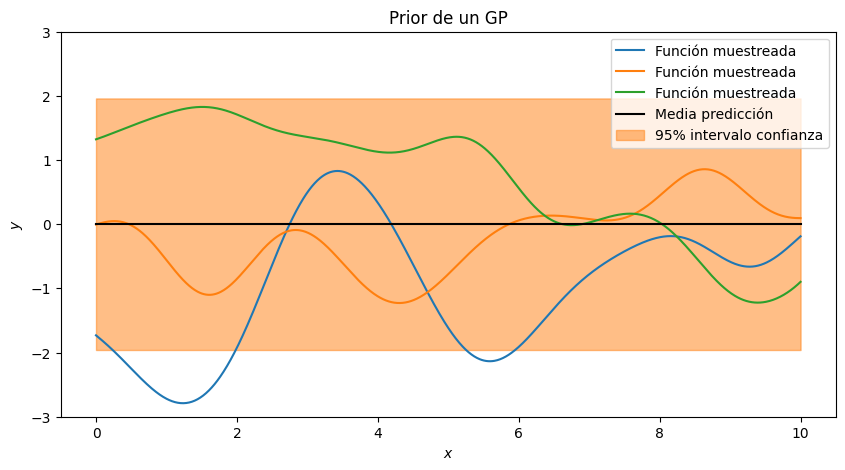
\includegraphics[trim={0cm 0cm 0cm 0cm},clip,width=\textwidth]{gpprior.png}
	\caption{Prior de un $\gp$. A modo ilustrativo se grafican 3 muestras del prior del $\gp$.}
	\label{fig:gprior}
\end{figure}


\subsubsection{Predicción \emph{posterior} sin ruido}
Supongamos que tenemos observaciones $(X,f(X))$ donde $X=\left(x_1,\dots,x_n\right)$ y queremos realizar una predicción sobre un conjunto de valores $X^*$ de tamaño $n^*$ ($X$ y $X^*$ pueden o no compartir valores). De la definición de $\gp$ se desprende inmediatamente que la distribución conjunta es:
\begin{align}
	\begin{bmatrix} f(X) \\ f(X^*)  \end{bmatrix}
	\sim \mathcal{N} \left(
	\begin{bmatrix} m(X) \\ m(X^*)  \end{bmatrix}, 
	\begin{bmatrix}
		K(X, X) & K(X, X^*) \\ K(X^*, X) & K(X^*, X^*)
	\end{bmatrix}
	\right)
\end{align}
Como para realizar la predicción necesitamos la distribución de $f(X^*)$ (condicional a los datos conocidos, por supuesto), nos valeremos del siguiente resultado:

\paragraph{Proposición:} dado un prior $\gp$, la posterior también es un $\gp$ y se puede condicionar sobre los datos conocidos para obtener:
\begin{equation}
	f(X^*) | f(X), X  \sim \mathcal{N}(m_{X^*|X}, \Sigma_{X^*|X}) \label{eq:gp_post}
\end{equation}
Donde la media y covarianza son:
\begin{align}
	m_{X^*|X} & = m(X^*) + K(X^*, X)K^{-1}(X, X) (f(X) - m(X))\\
	\Sigma_{X^*|X} & = K(X^*, X^*) - K(X^*, X)K^{-1}(X, X) K(X, X^*)
\end{align}


Observemos que tanto la media como la covarianza de la distribución de $f(X^*)$ dependen tanto de las observaciones conocidas (que juegan el papel de datos de entrenamiento) como de los valores de $X^*$ en donde deseamos realizar las predicciones $f(X^*)$.

Veamos un ejemplo de esto en acción. Supongamos nuevamente media cero y kernel $SE$ con $\sigma=l=1$. Tomemos a $X$ como 6 datos entre 0 y $10$, y las $f(X)$ dadas por $f(x)=x\sin(x)$. Tomemos ahora para predecir a $X^*$ como 100 datos equiespaciados entre $0$ y $10$. Realizamos 3 muestreos de la $f(X^*) | f(X), X$ que se pueden ver en la figura \ref{fig:gpostsinruido}.
\begin{figure}[H]
	\centering
	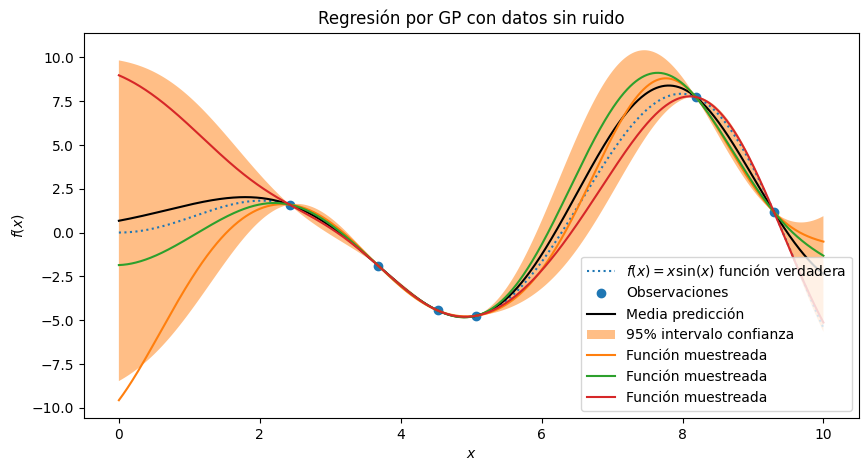
\includegraphics[trim={0cm 0cm 0cm 0cm},clip,width=\textwidth]{gppostsinruido.png}
	\caption{Regresión por $\gp$ con datos sin ruido. A modo ilustrativo se grafican 3 muestras del posterior del $\gp$.}
	\label{fig:gpostsinruido}
\end{figure}

Observemos que la predicción puede realizarse tanto interpolando como extrapolando a los datos conocidos. Además el intervalo de confianza es más angosto cuando los datos conocidos están menos distantes.



\subsubsection{Predicción \emph{posterior} con ruido}
En aplicaciones reales es normal tener mediciones con ruido. Supongamos que tenemos observaciones $(X,f(X))$ donde $X=\left(x_1,\dots,x_n\right)$, pero ahora nuestras observaciones tiene ruido $y_i = f(x_i) + \eta$, donde suponemos que $\eta \sim \mathcal{N}(0, \sigma^2_n)$ y que el ruido es i.i.d. Por lo tanto ahora nuestro conjunto de datos es de la forma $(X,Y)$ donde $Y=f(X) + \eta$. 

Es fácil ver que este ruido equivale, en nuestro modelo, a agregar un término diagonal a la covarianza:
$$ cov(Y) = K(X,X) + \sigma^2_n\mathbb{I} $$
Nuevamente queremos predecir sobre un conjunto $X^*$, y en este caso la conjunta queda como:
\begin{align}
	\begin{bmatrix} Y \\ f(X^*)  \end{bmatrix}
	\sim \mathcal{N} \left(
	\begin{bmatrix} m(X) \\ m(X^*)  \end{bmatrix}, 
	\begin{bmatrix}
		K(X,X) + \sigma_n^2\mathbb{I} & K(X, X^*) \\ K(X^*,X) & K(X^*,X^*)
	\end{bmatrix}
	\right)
\end{align}

Al igual que en el caso sin ruido tenemos un resultado sobre la distribución condicional que nos permite realizar predicciones:
\paragraph{Proposición:} 
	\begin{equation}
	f(X^*)|Y, X  \sim \mathcal{N}(m_{X^*|X}, \Sigma_{X^*|X})\label{eq:gp_posterior}
\end{equation}
Donde la media y covarianza son:
\begin{align}
	m_{X^*|X} & = m(X^*) + K(X^*, X) \left[K(X, X) + \sigma_n^2\mathbb{I}\right]^{-1} \left(Y - m(X)\right)\\
	\Sigma_{X^*|X} & = K(X^*, X^*) - K(X^*, X) \left[K(X, X) + \sigma_n^2\mathbb{I}\right]^{-1} K(X, X^*)
\end{align}

En la figura \ref{fig:gpostconruido} se puede ver este caso en acción, tomando los mismos parámetros y datos que para el ejemplo sin ruido, y tomando un ruido gaussiano de varianza 1.
\begin{figure}[H]
	\centering
	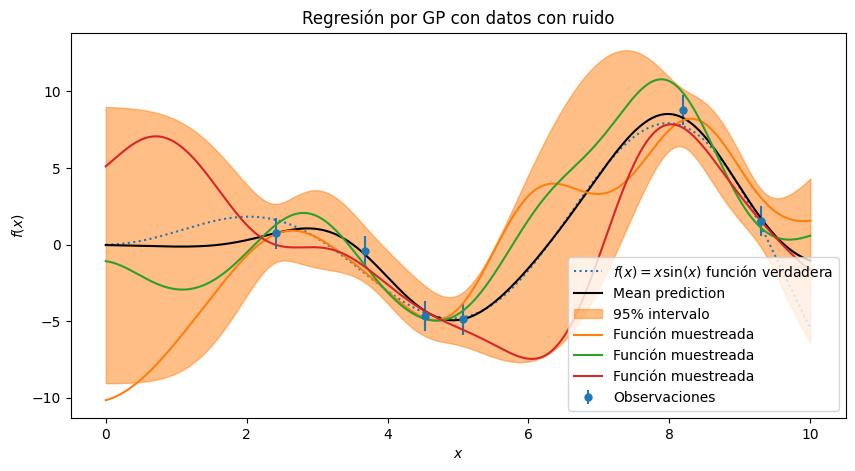
\includegraphics[trim={0cm 0cm 0cm 0cm},clip,width=\textwidth]{gppostconruido.png}
	\caption{Regresión por $\gp$ con datos \emph{con} ruido. A modo ilustrativo se grafican 3 muestras del posterior del $\gp$.}
	\label{fig:gpostconruido}
\end{figure}
Si comparamos la figura \ref{fig:gpostconruido} con la figura \ref{fig:gpostsinruido} observamos que ahora que los datos tienen ruido, la media de la gaussiana ya no necesariamente interpola a las observaciones (léáse no interpola la esperanza de las observaciones).



\section{Metodología}

\subsection{Datos: descripción, prepocesamiento y análisis exploratorio}
Como mencionamos en la sección \ref{sec:introd} los datos son de producción de petróleo y gas mensual desde 2006 publicada por la Secretaría de Energía de la Nación, abiertos y accesibles desde:\\

\url{https://datos.gob.ar/dataset/energia-produccion-petroleo-gas-por-pozo-capitulo-iv}\\

Estos datos tienen información mensual discriminada por pozo, a saber: producción de petróleo, gas y agua; inyección de agua, gas, CO$_2$ u otro; yacimiento, cuenca, concesión y provincia a la que pertenece; además de datos sobre la empresa operadora del pozo. En total son 971.882 datos.

Como primera medida se procedió a explorar la calidad de los datos, detectándose casos en donde una o más covariables tenían datos faltantes y esto derivaba en una mala carga del dato pues el faltante siempre ocurría en las covariables finales y, observando los demás datos de buena calidad, se podía deducir que había ocurro un ``corrimiento'' hacia las covariables primeras. Es decir, por poner un ejemplo, si el dato constaba de $x_1,\dots,x_9$ y $x_9$ tenía dato faltante, mirando datos de buena calidad, se podía deducir que el faltante en realidad estaba entrea las $x_1,\dots,x_8$ y no en la $x_9$. Este tipo de datos se descartaron, siendo su cantidad no significativa sobre el total, por la imposibilidad en muchos casos de identificar adecuadamente a cuál o cuáles covariables pertenecía el faltante.

Como uno de los objetivos de este trabajo será realizar predicciones sobre series temporales de la producción de petróleo y gas mensual, pero a primer acercamiento sin discriminar por pozo (ni por cuenca, provincia, etc.) entonces se procedió a sumar para cada mes la producción de todos los pozos, obteniéndose la producción mensual total de petróleo y gas. Cabe aclarar que un pozo puede, y en general lo hace, producir al mismo tiempo tanto petróleo como gas.

Como los procesos gaussianos que se desean usar en este trabajo son alimentados por series de datos ordenados, por ejemplo por el tiempo en el caso de producción de petróleo y gas, como ya se ejemplificó en la sección \ref{subsec:muestreoGP}, posterior a la obtención de la producción total por mes se procedió a inspeccionar los datos para corroborar que los mismos eran adecuados para usarse con la técnica antes mencionada. Las figuras \ref{fig:prodPet} y \ref{fig:prodGas} muestran la producción mensual desde Enero de 2006 hasta Marzo de 2023 de petróleo (en m$^3$) y de gas (en miles de m$^3$), comprobando que efectivamente estos datos sirven para alimentar a los procesos gaussianos descriptos en la sección \ref{subsec:introGP} y ejemplificados en la sección \ref{subsec:muestreoGP}.

\begin{figure}[h]
	\centering
	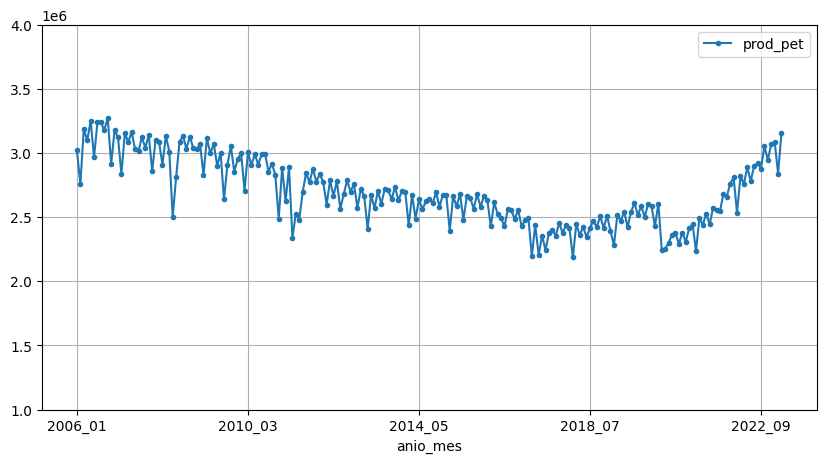
\includegraphics[trim={0cm 0cm 0cm 0cm},clip,width=\textwidth]{prod_pet.png}
	\caption{Producción total mensual de petróleo en m$^3$ en Argentina, desde Enero-2006 hasta Marzo-2023 según la Secretaría de Energía de la Nación.}
	\label{fig:prodPet}
\end{figure}

\begin{figure}[H]
	\centering
	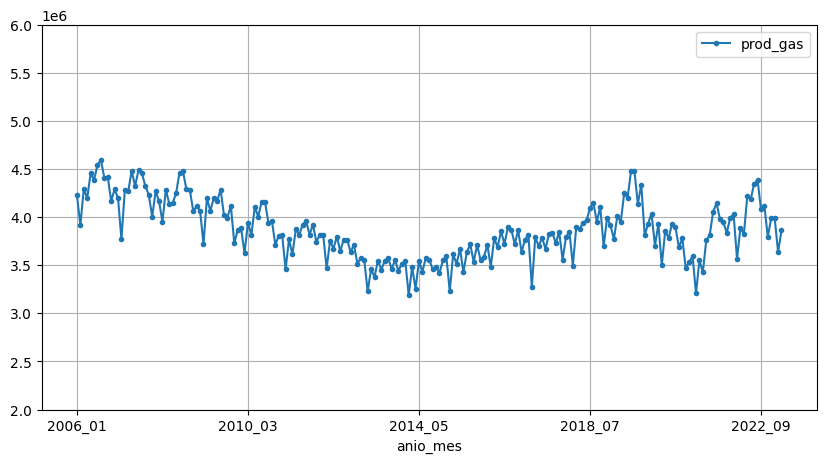
\includegraphics[trim={0cm 0cm 0cm 0cm},clip,width=\textwidth]{prod_gas.png}
	\caption{Producción total mensual de gas en miles de m$^3$ en Argentina, desde Enero-2006 hasta Marzo-2023 según la Secretaría de Energía de la Nación.}
	\label{fig:prodGas}
\end{figure}



\subsection{Técnicas de análisis y modelado}
\begin{itemize}
	\item Contar brevemente de nuevo el modelado de los datos, tanto de entrenamiento como de testeo, por una gaussiana multivariada, y contar brevemente de nuevo la técnica para predecir con $\gp$s descripta en \ref{subsec:muestreoGP}.
	
	\item Hablar sobre la medida de incertidumbre dada naturalmente por el $\gp$: la diagonal de la covarianza.
	
	\item Describir el o los diseños del kernel para esta serie de tiempo particular: término de tendencia a largo plazo, término de estacionalidad, término de irregularidades a corto plazo, ¿término de ruido?, ¿otros?. Hay un ejemplo interesante de esto en \url{https://scikit-learn.org/stable/auto_examples/gaussian_process/plot_gpr_co2.html#design-the-proper-kernel}.
	
	También se puede ver \cite{tesisduvenaud} y \url{https://www.cs.toronto.edu/~duvenaud/cookbook/}.
	
	Cada término es un kernel, y la suma de kernels es un kernel.
	
	\item ¿Acá o en Marco Teórico? Describir la influencia de los parámetros de cada kernel. Hablar de la optimización de los parámetros a partir de los datos (hay una explicación linda de esto en \cite{tobar}). Optimización de los parámetros: máxima verosimilitud y/o MCMC.
\end{itemize}



\section{Resultados y discusión}

\begin{itemize}
	\item Poner el resultado mínimo previo utilizando un kernel RBF.
	
	\item Si da el tiempo: probar con distintos kernels (leáse suma de) y con distintas ventanas de tiempo hacia atrás para predecir. Intuición: la ventana determina en cierta medida el kernel. Implicancias de la intuición: posible rediseño del kernel cada vez que se desea predecir.
	
	Se puede leer del cap. 2 de \cite{tesisduvenaud}. Una explicación más informal de lo mismo está en \url{https://www.cs.toronto.edu/~duvenaud/cookbook/}.
	
	\item Limitación: modelado gaussiano, diseño del kernel y optimización de sus parámetros.
	\item Limitación: los $\gp$ con poco eficientes en altas dimensiones. En algún lado leí que ya se complica si los features sobrepasan un par de decenas.
	\item Mejora: usar más features y no solamente el tiempo. Investigar sobre esto: por ahora es una inquietud más bien en el aire.
	\item Mejora: usar procesos gaussianos multi output. Intuición de esto: hacer uso de la correlación entre la producción de petróleo y de gas.
	\item Mejora: discriminar por zonas. Intuición de esto: cada zona tiene sus propios tiempos y volúmenes de producción.
	\item Mejora: discriminar por antigüedad de pozo y/o yacimiento. Intuición de esto: el volumen de producción está correlacionado a la antigüedad.
\end{itemize}



\section{Conclusiones}


\section{Ideas que todavía no puse en ningún lado}
\begin{itemize}
	\item Relacionar los modelos aditivos de series de tiempo clásicos: tendencia largo plazo + estacionalidad1 + estacionalidad2 + ... + irregularidades + ruido, con la aditividad de kernels. Intuición de esto: cada kernel modela un término del clásico.
	
	Idea general de esto: el $\gp$ es el análogo probabilístico al modelo clásico.
\end{itemize}


%\newpage
\begin{thebibliography}{9}
	
	\bibitem{gramacy}
	Robert B. Gramacy, \textit{Gaussian process modeling, design and optimization for the applied sciences},\\
	\url{https://bookdown.org/rbg/surrogates/}\\
	2023-03-05.
	
	\bibitem{tobar}
	Felipe Tobar, \textit{Aprendizaje de máquinas. Cap. 8: procesos gaussianos},\\
	\url{https://raw.githubusercontent.com/GAMES-UChile/Curso-Aprendizaje-de-Maquinas/master/notas_de_clase.pdf}\\
	2021.
	
	\bibitem{rasmussen}
	Carl E. Rasmussen; Christopher K. I. Williams, \textit{Gaussian Processes for Machine Learning},\\
	\url{http://gaussianprocess.org/gpml/}\\
	MIT Press, 2006.
	
	\bibitem{murphy}
	Kevin P. Murphy, \textit{Machine Learning: A Probabilistic Perspective. Ch. 15: Gaussian processes},\\
	\url{http://noiselab.ucsd.edu/ECE228/Murphy_Machine_Learning.pdf}\\
	MIT Press, 2012.
	
	\bibitem{hyndman}
	Rob J. Hyndman; George Athanasopoulos, \textit{Forecasting: Principles and Practice},\\
	\url{https://otexts.com/fpp3/}\\
	3ra. ed., 2021.
	
	\bibitem{gppaper1}
	Osaro, Etinosa; Okorie, Vivian; Alornyo, Sonia, \textit{Exploring the Usefulness of Gaussian Process Regression for the Prediction of Oil, Water and Gas Production Rates},\\
	Abril 2023, 14. 10.35248/2157-7463.23.14.506.\\
	\url{https://www.researchgate.net/profile/Etinosa-Osaro/publication/370099861_Exploring_the_Usefulness_of_Gaussian_Process_Regression_for_the_Prediction_of_Oil_Water_and_Gas_Production_Rates/links/643ed71a39aa471a5248f03a/Exploring-the-Usefulness-of-Gaussian-Process-Regression-for-the-Prediction-of-Oil-Water-and-Gas-Production-Rates.pdf}
	
	\bibitem{tesisduvenaud}
	David K. Duvenaud, \textit{Automatic Model Construction with Gaussian Processes},\\
	\url{https://www.cs.toronto.edu/~duvenaud/thesis.pdf}\\
	PhD thesis, 2014, University of Cambridge.
	
\end{thebibliography}


\end{document}
